\documentclass{article}
\usepackage{geometry}
\geometry{
	a4paper,
	left=2.5cm,   
	right=2.5cm,   
	top=2.5cm,      
	bottom=2.5cm,  
	headheight=13.6pt
}

% 字体设置（需使用 XeLaTeX 编译）
\usepackage{fontspec}
\usepackage[UTF8, fontset=none]{ctex}

% 设置英文默认字体为 Times New Roman
\setmainfont{Times New Roman}[
BoldFont = Times New Roman Bold,
ItalicFont = Times New Roman Italic,
BoldItalicFont = Times New Roman Bold Italic
]

% 手动设置中文字体
\setCJKmainfont{SimSun}[
BoldFont = SimHei,
ItalicFont = KaiTi
]
\setCJKsansfont{SimHei}
\setCJKmonofont{FangSong}

\usepackage{amsmath}
\usepackage{amssymb}
\usepackage{booktabs}
\usepackage{caption}
\usepackage{setspace}
\usepackage{array}
\usepackage{listings}
\usepackage{graphicx}
\usepackage{enumitem}
\usepackage{subcaption}
\usepackage{multirow}
\usepackage{xcolor}
\usepackage{colortbl}

% 定义代码颜色
\definecolor{codegreen}{rgb}{0,0.6,0}
\definecolor{NavyBlue}{RGB}{0,0,128}
\definecolor{PineGreen}{RGB}{1,121,111}

% 配置 listings 环境
\lstset{
	language=Python,
	tabsize=4,
	captionpos=b,
	numbers=left,
	numbersep=1em,
	sensitive=true,
	showtabs=false,
	frame=shadowbox,
	breaklines=true,
	keepspaces=true,
	showspaces=false,
	showstringspaces=false,
	breakatwhitespace=false,
	basicstyle=\ttfamily\small,
	keywordstyle=\color{NavyBlue},
	commentstyle=\color{codegreen},
	numberstyle=\color{black},  % 将 gray 改为 black
	stringstyle=\color{PineGreen!90!black},
	rulesepcolor=\color{red!20!green!20!blue!20}
}

\definecolor{LightGreen}{rgb}{0.9, 0.95, 0.9}
\definecolor{LightBlue}{RGB}{229, 238, 255}
\definecolor{LightPink}{RGB}{255, 229, 237}

% 表格标题格式：字体为黑体
\captionsetup[table]{
	labelsep=quad,
	font={bf}
}

% 设置图片标题（图注）字体为黑体
\captionsetup[figure]{
	labelsep=quad,
	font={bf}
}

% 设置子图标题字体为黑体
\captionsetup[subfigure]{
	font={bf}
}

\begin{document}
	
	\begin{center}
		{\LARGE \textbf{数学模型作业}} \\[0.5cm]
		{\large 石继楷 \quad 202411079123} \\[0.3cm]
		{\large 2026年5月28日}
	\end{center}
	
	\section{作业1：Logistic 微分方程求解}
	
	\noindent
	由题：
	\( \displaystyle
	\frac{dN}{dt} = r\left(1-\frac{N}{K}\right)N,\quad N(0)=N_0
	\)
	
	\vspace{0.3cm}
	\noindent
	分离变量：
	\( \displaystyle \frac{dN}{N\left(1-\frac{N}{K}\right)} = r\,dt\)
	
	\vspace{0.3cm}
	\noindent
	\(\therefore \displaystyle \int \left( \frac{1}{N}+\frac{1}{K-N} \right) dN
	= \int r\,dt\)
	
	\vspace{0.3cm}
	\noindent
	\(\therefore \displaystyle \ln|N| - \ln|K-N| = rt + C\)
	
	\vspace{0.3cm}
	\noindent
	\(\therefore \displaystyle \frac{N}{K-N}=Ce^{rt}\)
	
	\vspace{0.3cm}
	\noindent
	代入初始条件 \(t=0,\ N=N_0\)，得 \(C=\dfrac{N_0}{K-N_0}\)
	
	\vspace{0.3cm}
	\noindent
	\(\therefore \displaystyle N(t)=\frac{K}{1+\left(\frac{K}{N_0}-1\right)e^{-rt}}\)
	
	\section{作业2：人口模型拟合}
	
	关键拟合代码：
	
	\begin{lstlisting}[language=Python, basicstyle=\small\ttfamily]
def malthus(t, N0, r):
return N0 * np.exp(r * t)                   # Malthus指数增长模型
def logistic(t, K, N0, r):
return K / (1 + (K/N0 - 1) * np.exp(-r * t))  # Logistic阻滞增长模型
def fit_malthus(t, pop):
N0_init = pop[0]                            # 初始人口
r_init = np.log(pop[-1]/pop[0]) / (t[-1] - t[0])  # 增长率初值
params, _ = curve_fit(malthus, t, pop, p0=[N0_init, r_init])
return params
def fit_logistic(t, pop):
N0_init = pop[0]                            # 初始人口
K_init = pop[-1] * 1.5                      # 环境容纳量初值
r_init = np.log(pop[-1]/pop[0]) / (t[-1] - t[0])  # 增长率初值
params, _ = curve_fit(logistic, t, pop, p0=[K_init, N0_init, r_init],
bounds=(0, [np.inf, np.inf, np.inf]))  # 非负约束
return params
def compute_r2(actual, pred):
return 1 - np.sum((actual - pred)**2) / np.sum((actual - np.mean(actual))**2)#R²\end{lstlisting}
	
	\subsection{美国人口拟合（1790--2020，单位：百万）}
	\begin{table}[htbp]
		\centering
		\caption{美国1790—2020年人口数据（单位：百万）}
		\renewcommand{\arraystretch}{1.2}
		\renewcommand{\heavyrulewidth}{1.2pt}
		\setlength{\tabcolsep}{3em}
		\begin{tabular}{cccc}
			\toprule
			年份 & 人口 & 年份 & 人口 \\
			\midrule
			1790 & 3.9  & 1910 & 92.0  \\
			1800 & 5.3  & 1920 & 106.5 \\
			1810 & 7.2  & 1930 & 123.2 \\
			1820 & 9.6  & 1940 & 131.7 \\
			1830 & 12.9 & 1950 & 150.7 \\
			1840 & 17.1 & 1960 & 179.3 \\
			1850 & 23.2 & 1970 & 204.0 \\
			1860 & 31.4 & 1980 & 226.5 \\
			1870 & 38.6 & 1990 & 251.4 \\
			1880 & 50.2 & 2000 & 282.2 \\
			1890 & 62.9 & 2010 & 308.7 \\
			1900 & 76.0 & 2020 & 331.4 \\
			\bottomrule
		\end{tabular}
		\renewcommand{\heavyrulewidth}{0.8pt}
	\end{table}
	
	\begin{figure}[h!]
		\centering
		\subcaptionbox{美国人口使用Malthus模型拟合}{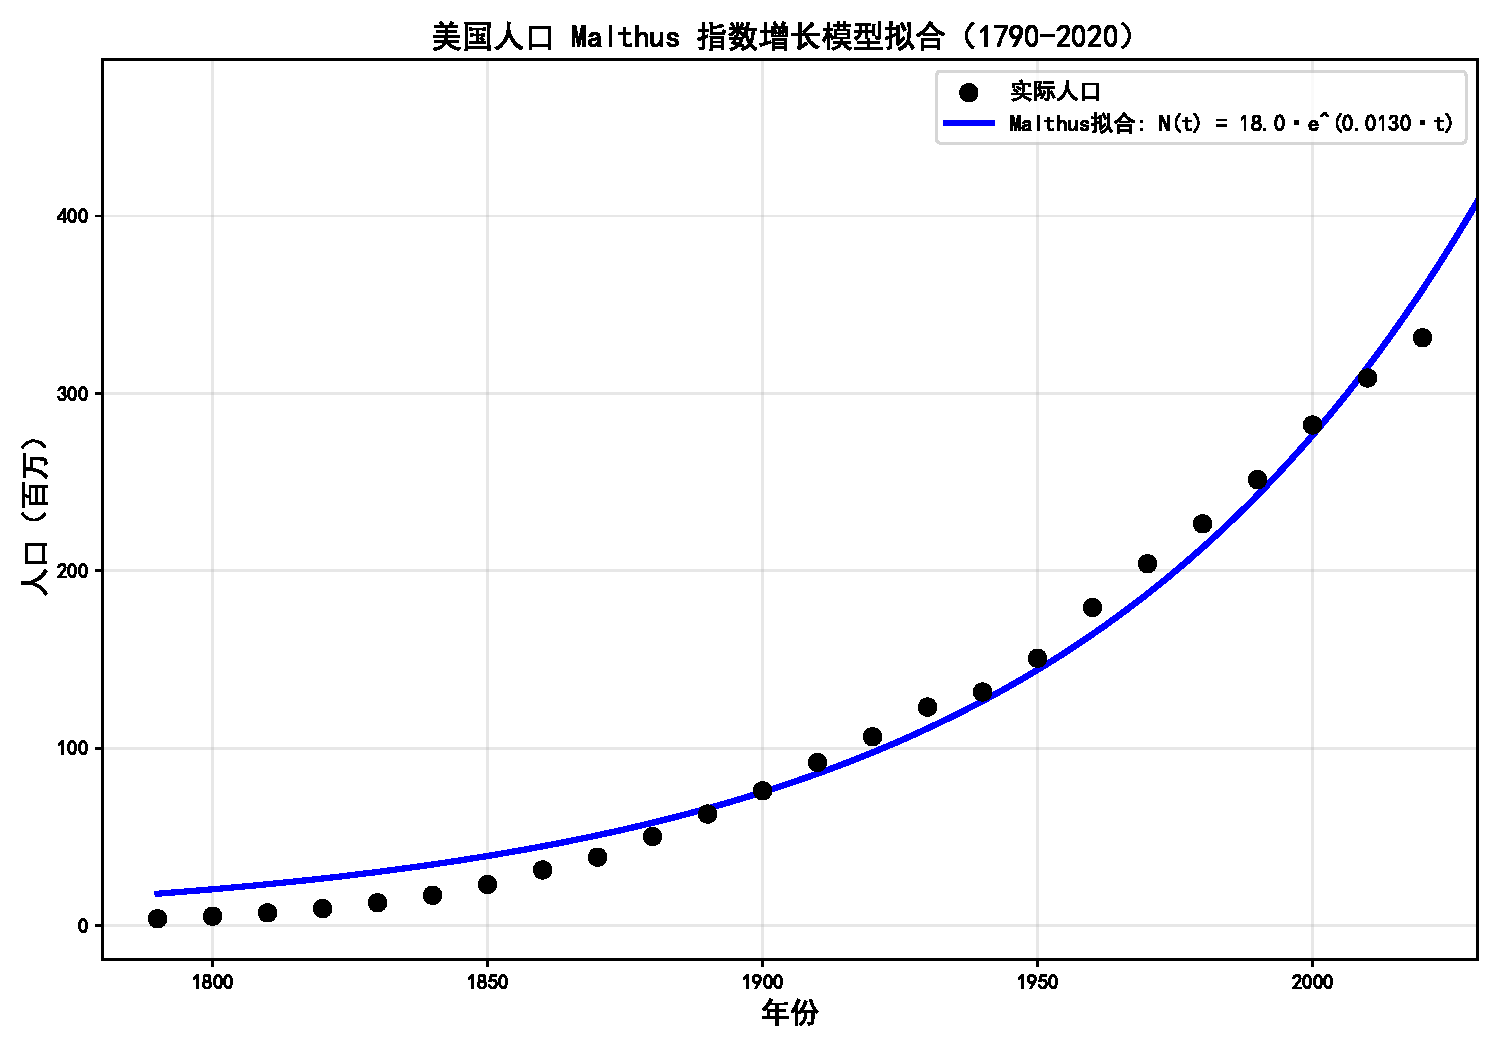
\includegraphics[width=.45\textwidth]{figures/美国Malthus}}%
		\hfill
		\subcaptionbox{美国人口使用Logistic模型拟合}{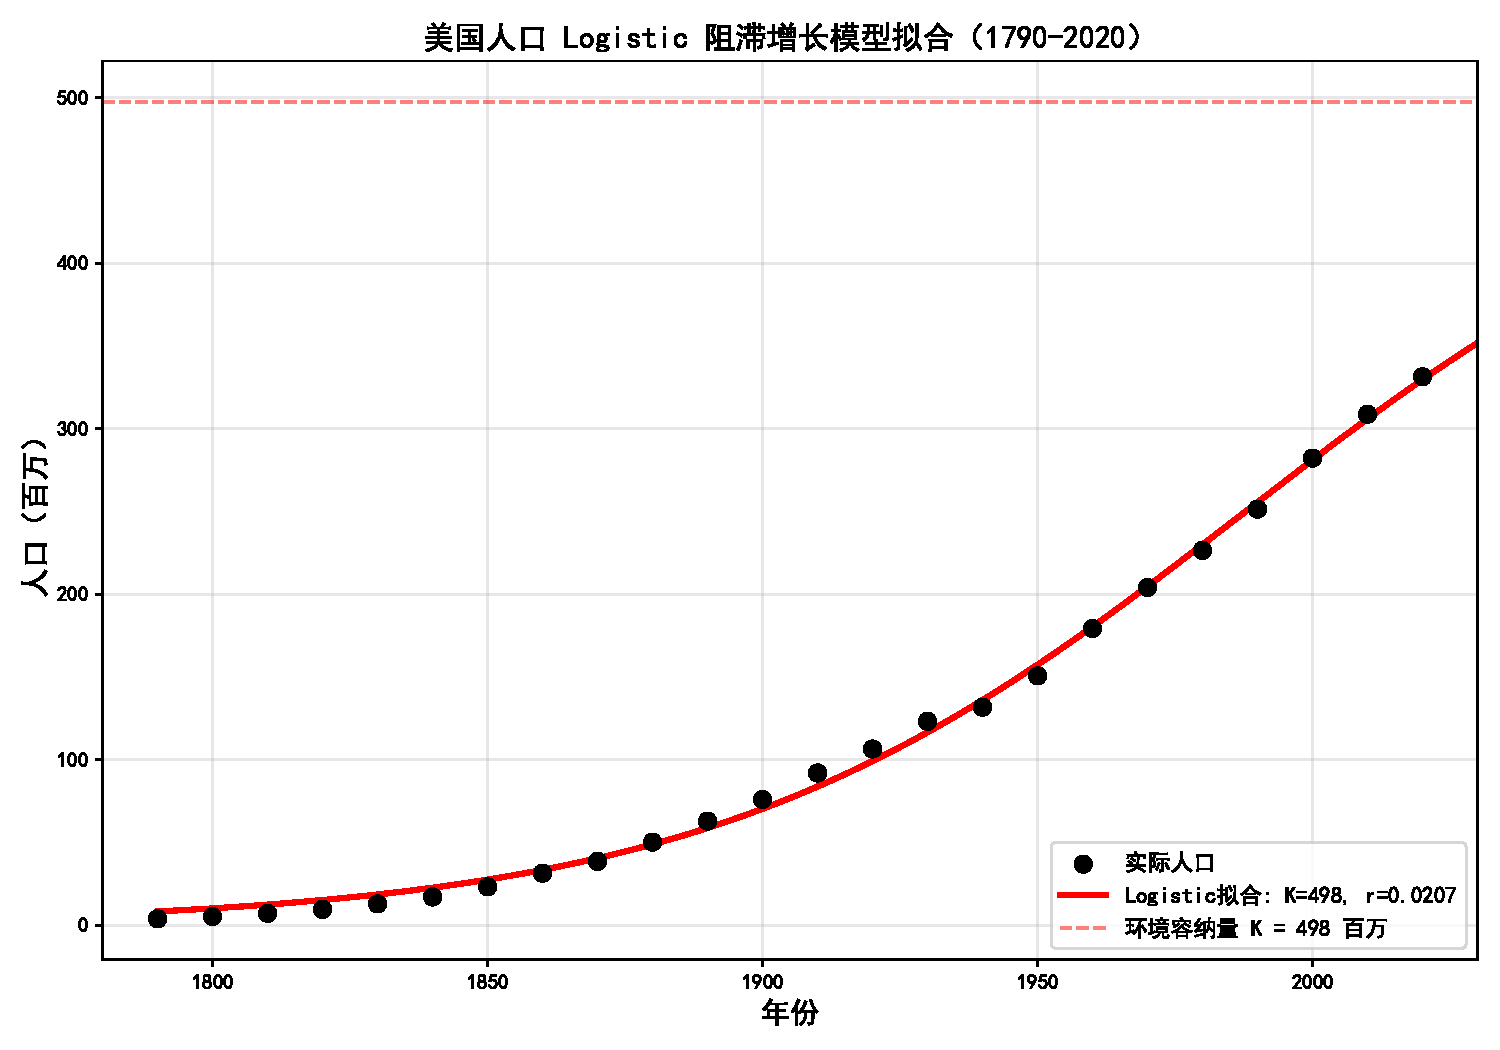
\includegraphics[width=.45\textwidth]{figures/美国Logistic}}
		\caption{美国人口的两种模型拟合}
		\label{fig:美国}
	\end{figure}
	
	\begin{table}[htbp]
		\centering
		\setlength{\tabcolsep}{8pt}
		\renewcommand{\arraystretch}{1.3}
		\caption{美国人口模型拟合结果对比}
		\label{tab:usa_pop_fit}
		\begin{tabular}{lcccc}
			\toprule
			\textbf{模型类型} & \textbf{初始人口 }\(N_0\) & \textbf{增长率 }\(r\) & \textbf{环境容纳量 }\(K\) & \textbf{\(R^2\)} \\
			\midrule
			Malthus模型 & 17.98 & 0.0130 & -- & 0.9837 \\
			Logistic模型 & 8.30 & 0.0207 & 497.6 & 0.9980 \\
			\bottomrule
		\end{tabular}
	\end{table}
	
	从拟合结果可以看出，Logistic模型的\(R^2=0.9980\)显著高于Malthus模型的\(R^2=0.9837\)，且RMSE仅为4.63百万，远小于Malthus模型的13.15百万。这说明Logistic模型能更准确地描述美国人口的增长规律。美国的人口环境容纳量约为4.98亿，符合预期。
	
	\newpage
	\subsection{中国人口拟合（2000--2020，单位：亿）}
	
	\begin{table}[htbp]
		\centering
		\caption{中国2000—2020年人口数据（单位：亿）}
		\renewcommand{\arraystretch}{1.2}
		\renewcommand{\heavyrulewidth}{1.2pt}
		\setlength{\tabcolsep}{3em}
		\begin{tabular}{cccc}
			\toprule
			年份 & 人口 & 年份 & 人口 \\
			\midrule
			2000 & 12.6743 & 2011 & 13.4735 \\
			2001 & 12.7627 & 2012 & 13.5404 \\
			2002 & 12.8453 & 2013 & 13.6072 \\
			2003 & 12.9227 & 2014 & 13.6782 \\
			2004 & 12.9988 & 2015 & 13.7462 \\
			2005 & 13.0756 & 2016 & 13.8271 \\
			2006 & 13.1448 & 2017 & 13.9008 \\
			2007 & 13.2129 & 2018 & 13.9538 \\
			2008 & 13.2802 & 2019 & 14.0005 \\
			2009 & 13.3450 & 2020 & 14.1178 \\
			2010 & 13.4091 &  &  \\
			\bottomrule
		\end{tabular}
		\renewcommand{\heavyrulewidth}{0.8pt}
	\end{table}
	
	\begin{figure}[h!]
		\centering
		\subcaptionbox{中国人口使用Malthus模型拟合}{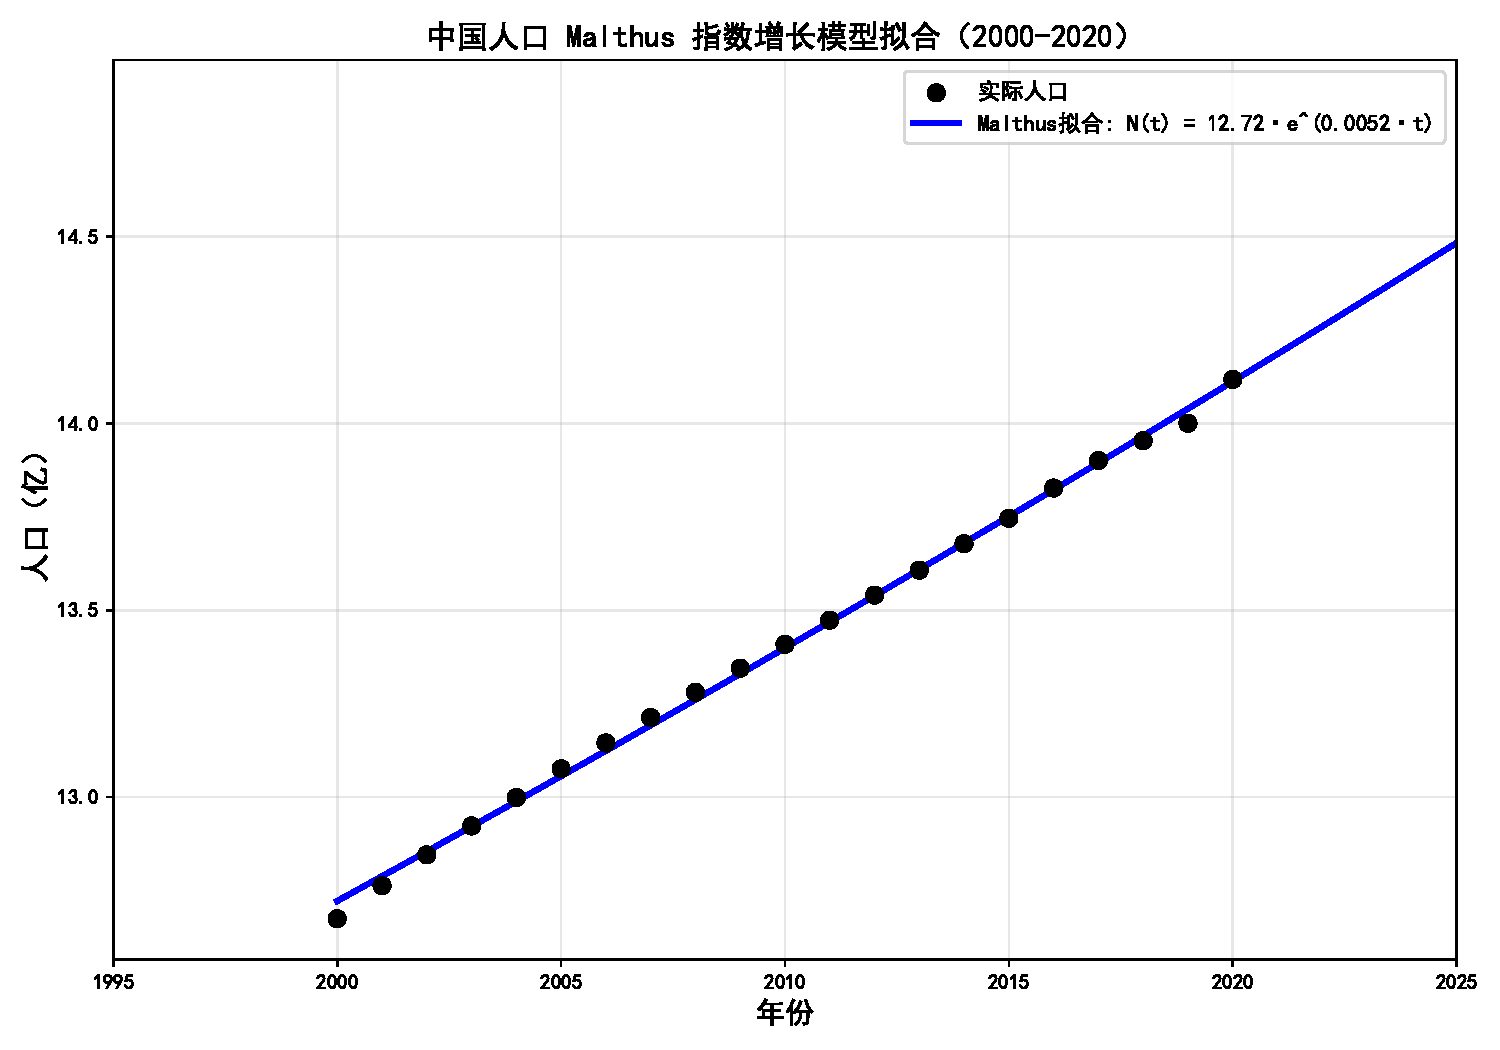
\includegraphics[width=.45\textwidth]{figures/中国Malthus}}%
		\hfill
		\subcaptionbox{中国人口使用Logistic模型拟合}{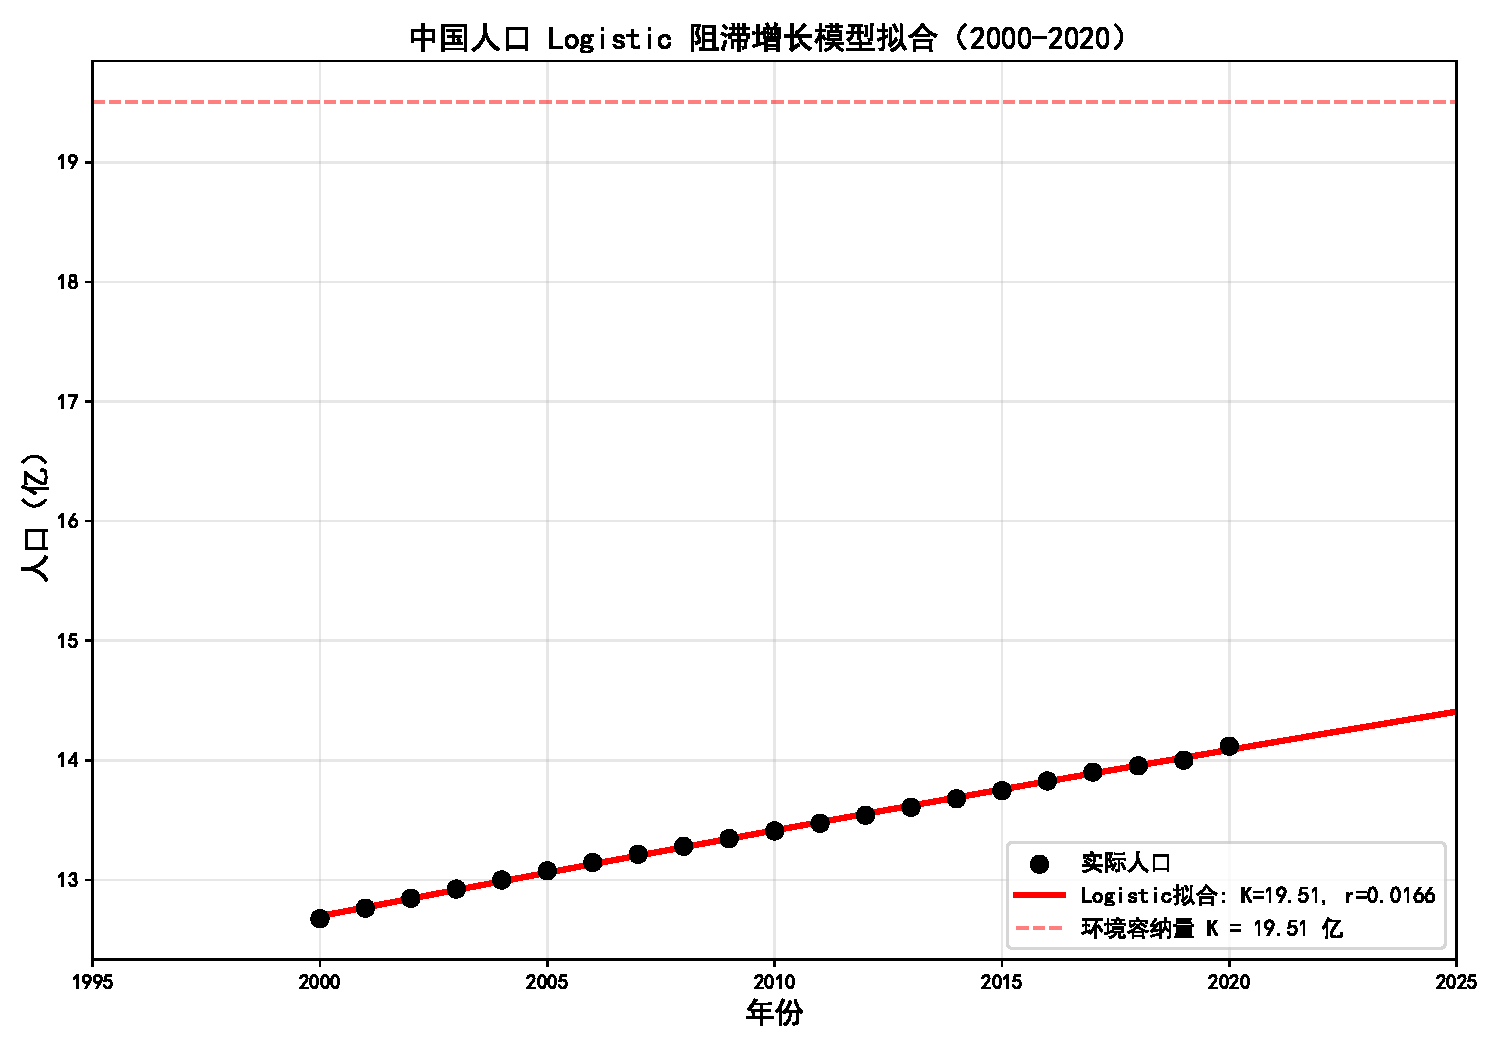
\includegraphics[width=.45\textwidth]{figures/中国Logistic}}
		\caption{中国人口的两种模型拟合}
		\label{fig:中国}
	\end{figure}
	
	\begin{table}[htbp]
		\centering
		\setlength{\tabcolsep}{8pt}
		\renewcommand{\arraystretch}{1.3}
		\caption{中国人口模型拟合结果对比}
		\label{tab:chn_pop_fit}
		\begin{tabular}{lcccc}
			\toprule
			\textbf{模型类型} & \textbf{初始人口 }\(N_0\) & \textbf{增长率 }\(r\) & \textbf{环境容纳量 }\(K\) & \textbf{\(R^2\)} \\
			\midrule
			Malthus模型 & 12.72 & 0.0052 & -- & 0.9982 \\
			Logistic模型 & 12.70 & 0.0166 & 19.51 & 0.9991 \\
			\bottomrule
		\end{tabular}
	\end{table}
	
	中国人口拟合结果显示，两个模型的\(R^2\)均超过0.998，拟合精度都很高。但Malthus模型的增长率\(r=0.0052\)表明人口将按指数持续增长，这忽略了资源环境的限制。Logistic模型给出的环境容纳量\(K=19.51\)亿，表明中国人口峰值约为19.5亿，且拟合的\(R^2=0.9991\)略优于Malthus模型。
	
	\subsection{拟合结论}
	
	综合两国人口数据的拟合结果，可以得到以下结论：
	
	\begin{enumerate}
		\item Malthus模型假设人口按指数增长，增长率\(r\)恒定。该模型形式简单，在人口增长早期或短期内拟合效果较好（两国\(R^2\)均大于0.98）。但其无法反映人口增长放缓的趋势，长期预测会严重偏离实际。
		
		\item Logistic阻滞增长模型考虑了资源环境对人口增长的限制，引入了环境容纳量\(K\)。该模型更符合人口增长的S型曲线特征：
		\begin{itemize}
			\item 美国人口环境容纳量\(K\approx 498\)百万，Logistic模型的\(R^2=0.9980\)，RMSE仅为4.63，远优于Malthus模型。
			\item 中国人口环境容纳量\(K\approx 19.5\)亿，Logistic模型的\(R^2=0.9991\)，拟合精度最高。
		\end{itemize}
		
		\item 从评价指标来看，Logistic模型在两个国家的拟合中均取得了更高的\(R^2\)和更低的RMSE，说明考虑了资源约束的阻滞增长模型更能反映真实的人口演化规律。Malthus模型仅适用于资源约束不明显的初期阶段，而Logistic模型更适合中长期人口预测。
	\end{enumerate}
	
	\section{作业3：利用Logistic模型迭代求数值解}
	
	以下为利用Logistic模型迭代计算得到数值结果的Python代码：
	
	\begin{lstlisting}[language=Python, basicstyle=\small\ttfamily]
b_values=[1.7,2.6,3.3,3.45,3.55]  # 题目给定的b参数列表
x0=0.2                           # 迭代初始值x0

result=[]                        # 存储所有b值对应的迭代结果
for b in b_values:                # 遍历每一个b值
seq=[x0]                      # 初始化当前b的迭代序列，存入初始值
x=x0                          # 将当前迭代值设为初始值
for _ in range(100):          # 迭代计算100次（生成0~100共101个值）
x=b*x*(1-x)               # Logistic迭代公式：x_{k+1}=b*x_k*(1-x_k)
seq.append(x)             # 将新迭代值加入序列
result.append(seq)            # 把当前b的完整序列存入总结果

print("k\tb=1.7\tb=2.6\tb=3.3\tb=3.45\tb=3.55")  # 打印表头
for k in range(101):              # 遍历0到100所有迭代步数
line=f"{k}"                   # 拼接当前步数k
for i in range(len(b_values)):  # 遍历每个b值对应的迭代结果
line+=f"\t{result[i][k]:.4f}"  # 拼接对应数值，保留4位小数
print(line)                   # 打印完整一行数据
\end{lstlisting}
	
\end{document}